% This is the ADASS_template.tex LaTeX file, 17th Jun 2019.
% It is based on the ASP general author template file, but modified to reflect the specific
% requirements of the ADASS proceedings.
% Copyright 2014, Astronomical Society of the Pacific Conference Series
% Revision:  14 August 2014

% To compile, at the command line positioned at this folder, type:
% latex ADASS_template
% latex ADASS_template
% dvipdfm ADASS_template
% This will create a file called ADASS_template.pdf

\documentclass[11pt,twoside]{article}
% Do NOT use ANY packages other than asp2014. 
\usepackage{asp2014}
\usepackage{draftwatermark}
\aspSuppressVolSlug
\resetcounters

\SetWatermarkAngle{0} 
% Color of the watermark
%\SetWatermarkColor{}
% Lightness   of   the   watermark   text(1=white, 0=black)
%\SetWatermarkLightness{〈real〉}
%Font size of the watermark text
\SetWatermarkFontSize{20pt}
%Scaling of the watermark text
%\SetWatermarkScale{〈real〉}
%Horizontal center of watermark text
\SetWatermarkHorCenter{13.0cm}
%Vertical center of watermark text
\SetWatermarkVerCenter{2cm}
%Watermark text
\SetWatermarkText{Draft-v29.10.2019.13:22 for comments}

% References must all use BibTeX entries in a .bibfile.
% References must be cited in the text using \citet{} or \citep{}.
% Do not use \cite{}.
% See ManuscriptInstructions.pdf for more details
\bibliographystyle{asp2014}

% The ``markboth'' line sets up the running heads for the paper.
% 1 author: "Surname"
% 2 authors: "Surname1 and Surname2"
% 3 authors: "Surname1, Surname2, and Surname3"
% >3 authors: "Surname1 et al."
% Replace ``Short Title'' with the actual paper title, shortened if necessary.
% Use mixed case type for the shortened title
% Ensure shortened title does not cause an overfull hbox LaTeX error
% See ASPmanual2010.pdf 2.1.4  and ManuscriptInstructions.pdf for more details
\markboth{Singh, Valentijn, Roerdink, Belikov and Buddelmeijer}{Distributed Visualization of Big Data}

\begin{document}

\title{Scientific Visualization of Extremely Large Distributed Astronomical Surveys}

% Note the position of the comma between the author name and the 
% affiliation number.
% Authors surnames should come after first names or initials, eg John Smith, or J. Smith.
% Author names should be separated by commas.
% The final author should be preceded by "and".
% Affiliations should not be repeated across multiple \affil commands. If several
% authors share an affiliation this should be in a single \affil which can then
% be referenced for several author names. If only one affiliation, no footnotes are needed.
% See ManuscriptInstructions.pdf and ASP's manual2010.pdf 3.1.4 for more details
\author{S.\,Singh,$^{1}$  E.\,A.\,Valentijn,$^1$ J.\,Roerdink,$^1$ A.\,Belikov,$^1$ and  H.\,Buddelmeijer$^{1}$}
\affil{$^1$Faculty of Science and Engineering, University of Groningen, the Netherlands; \email{rnsweta@gmail.com}}
%\affil{$^2$Anchormen B.V, Amsterdam, the Netherlands}
% This section is for ADS Processing.  There must be one line per author. paperauthor has 9 arguments.
\paperauthor{Sweta Singh}{rnsweta@gmail.com}{ORCID_Or_Blank}{RUG}{Kapteyn Astronomical Institute}{Groningen}{Groningen}{9747AD}{The Netherlands}
\paperauthor{Edwin A. Valentijn}{valentyn@astro.rug.nl}{ORCID_Or_Blank}{RUG}{Kapteyn Astronomical Institute}{Groningen}{Groningen}{9747AD}{The Netherlands}
\paperauthor{Andrey Belikov}{rnsweta@gmail.com}{belikov@astro.rug.nl}{RUG}{Kapteyn Astronomical Institute}{Groningen}{Groningen}{9747AD}{The Netherlands}
\paperauthor{Hugo Buddelmeijer}{buddel@astro.rug.nl}{ORCID_Or_Blank}{RUG}{Kapteyn Astronomical Institute}{Groningen}{Groningen}{9747AD}{The Netherlands}

% There should be one \aindex line (commented out) for each author. These are used to
% build up the author index for the Proceedings. The surname must come first, followed by
% initials. Note the use of ~ before each initial to control spacing.
% The \author entries (see above) have surname last. These \aindex entries have
% surname first.
% The Aindex.py command willl create them for you after you have constructed the \author
% The first entry should be the first author, for bold-facing the author index page-reference

%\aindex{Singh,~S.}
%\aindex{Valentijn,~Edwin~A.}
%\aindex{Belikov,~A.}
%\aindex{Buddelmeijer,~H.}


\begin{abstract}
Interactive real time visualization of large data sets is one of the core requirements for carrying out scientific
research. Its even more relevant for astronomy where new cutting edge large
telescopes will generate multi Peta Bytes\,(PB) sky surveys. We describe our solution, developed in context of the Euclid space mission whose large astronomical
imaging data would need to be distributed over several heterogeneous Science Data Centers\,(SDCs) across the world. In our distributed visualization architecture,
millions of survey images\,(HiPS) distributed over SDCs are efficiently
transported and combined to deliver image(s) of interest at the desired resolution (up to pixel level) to the user. This is achieved by optimally utilizing a combination of  several modern
tools consisting of {\it{http}} servers, Front-End Node and load-balancer\,(FEN), reverse proxies, PHP/Python scripts, MySQL databases, including on
the fly image generation/combination which all feed (only) the required information to the Aladin
interactive visualization tool at the remote user's Personal Computer\,(PC).
It has potential applications for other large projects\,(e.g. SKA)  with their data distributed across several locations due to its sheer size
or/and due to collaborative nature of the work.

\end{abstract}


% These lines show examples of subject index entries. At this stage these have to commented
% out, and need to be on separate lines. Eventually, they will be automatically uncommented
% and used to generate entries in the Subject Index at the end of the Proceedings volume.
% Don't leave these in! - replace them with ones relevant to your paper.
%\ssindex{FOOBAR!conference!ADASS 2019}
%\ssindex{FOOBAR!organisations!ASP}

% These lines show examples of ASCL index entries. At this stage these have to commented
% out, and need to be on separate lines. Eventually, they will be automatically uncommented
% and used to generate entries in the ASCL Index at the end of the Proceedings volume.
% The ascl.py command will scan your paper on possible code names.
% Don't leave these in! - replace them with ones relevant to your paper.
%\ooindex{FOOBAR, ascl:1101.010}


\section{Introduction}
Euclid (\url{http://sci.esa.int/euclid}) is an space mission led by Europe with the main scientific objective of carrying out visible and near infrared surveys of the entire extra-galactic sky  to improve our knowledge about the nature and structure  of dark contents of the universe.  Due to its unprecedented accuracy similar to that of the Hubble space telescope (\url{https://hubblesite.org}) and almost full sky coverage,  Euclid data would be of extreme value for almost all astronomical studies.  %While the 200\,Tera Byte\,(TB) of compressed telemetry data directly coming out of the Euclid space craft is modest by today's standard, it would be expanded by several factors of tens in the course of data analysis.
 The Euclid consortium (\url{https://www.euclid-ec.org}) has organized the scientific and technical community into a number of working groups for efficient workload distribution. The resulting data volume in excess of  few tens of PB  \citep{2017IAUS..325...73D} will be distributed over  several SDCs\,(in Europe, USA)  responsible for assigned functions. 

%In  such  large projects like Euclid, it may not be possible (or even desirable given the collaborative nature of the project) to store the entire data set at one physical location.
%{\noindent \emph { The need for distributed visualization:}}\, 
One of the main outputs at each of these SDCs would be high quality astronomical survey images and source catalogues.  The term images refers to  images from Euclid, related ground based telescopes and  simulation studies. The traditional approach involving local copy at users PCs or  large compute cluster, or even at one given physical location may  be difficult due to large data volumes and costs involved. It may not even be desirable given the collaborative nature and shared responsibilities in the project. Thus distributed, real time interactive visualization of the survey is critical to gain much needed insight for its effective harnessing to maximize  scientific astronomical research. 

%% Reference Example Check .. More is in Section \nameref{secn:dvp} and Section\,\ref{secn:dvp}.
\section{Distributed Visualization Pipeline}
\label{secn:dvp}

The two ends of any visualization pipeline framework are (i)\,{\emph {The Demand (User) Side}\,:} - \,the visualization software at the users end (client) and (ii)\,{\emph {The Supply Side}\,:} - a cohesive data storage, management and transport framework able to provide the required data/information in real time in an efficient and transparent manner. 

For Euclid, Aladin sky atlas (\url{https://aladin.u-strasbg.fr}) would be the main  visualization analysis tool on the user\,(client) side  (e.g. an astronomer). %Aladin allows users to interactively visualize digitized astronomical images\,(including all sky surveys), superimpose/overlay images, catalogues of other wave bands including interactively access related data and information from the Simbad (\url{http://simbad.u-strasbg.fr/simbad}) database, the Vizier (\url{https://vizier.u-strasbg.fr})  service and other archives for all known astronomical objects in the field.   
The default format for Euclid surveys would be based on Hierarchical Progressive Surveys\,(HiPS). HiPS  makes use of the hierarchical features of HEALPix to organise astronomical data into HEALPix maps of different orders/resolutions\,\citep{2015A&A...578A.114F}. The curvilinear partitioning of the sphere in HEALPix supports a hierarchical tree structure enabling multi-resolution applications\,\citep{2005ApJ...622..759G}. This multi-layer visualization with increasing angular resolution for each layer has similarities with Google Maps). 
%HiPS is also being successfully utilized for several projects including space missions for Astronomy (e.g. Planck4 (\url{https://sci.esa.int/web/planck}) and Gaia5 (\url{https://sci.esa.int/web/gaia}) space missions). 
%The merits behind the choice of Aladin and HiPS as the visualization tool and survey image format for Euclid is beyond the scope of the present study.  

We followed a two pronged approach, the first one being to develop a distributed visualization framework  to address the challenges at the  supply side of the visualization pipeline.   Secondly we also worked on ways to reduce the size of survey data itself. In this paper we  present only the work related to framework for  distributed visualization.

\section{Architectural Design}
\label{secn:arch_design}
The {\it{http}} compliant nature  of the HiPS  (\url{http://www.ivoa.net/documents/HiPS}) allows it to be  accessed via any {\it{http}} compliant server. We make use of this extremely useful feature to arrive at a client-server based  architectural design which binds the distributed resources across the SDCs into the distributed visualization framework. This flexible client-server  architecture also empowers us to utilize the {\it{http}} protocols and wide variety of available tools. As an example while the HiPS format does prescribe the storage of the HiPS image\,(survey) in a simple hierarchy of directory and files, the {\it{http}} compliance allows the actual storage behind the {\it{http}} server to be implemented in any desired manner provided the critical requirement of supplying the requested information to the client\,(e.g. Aladin) is correctly met. 
\begin{figure}[ht]
    \centering
%    \noindent\makebox[\textwidth]
   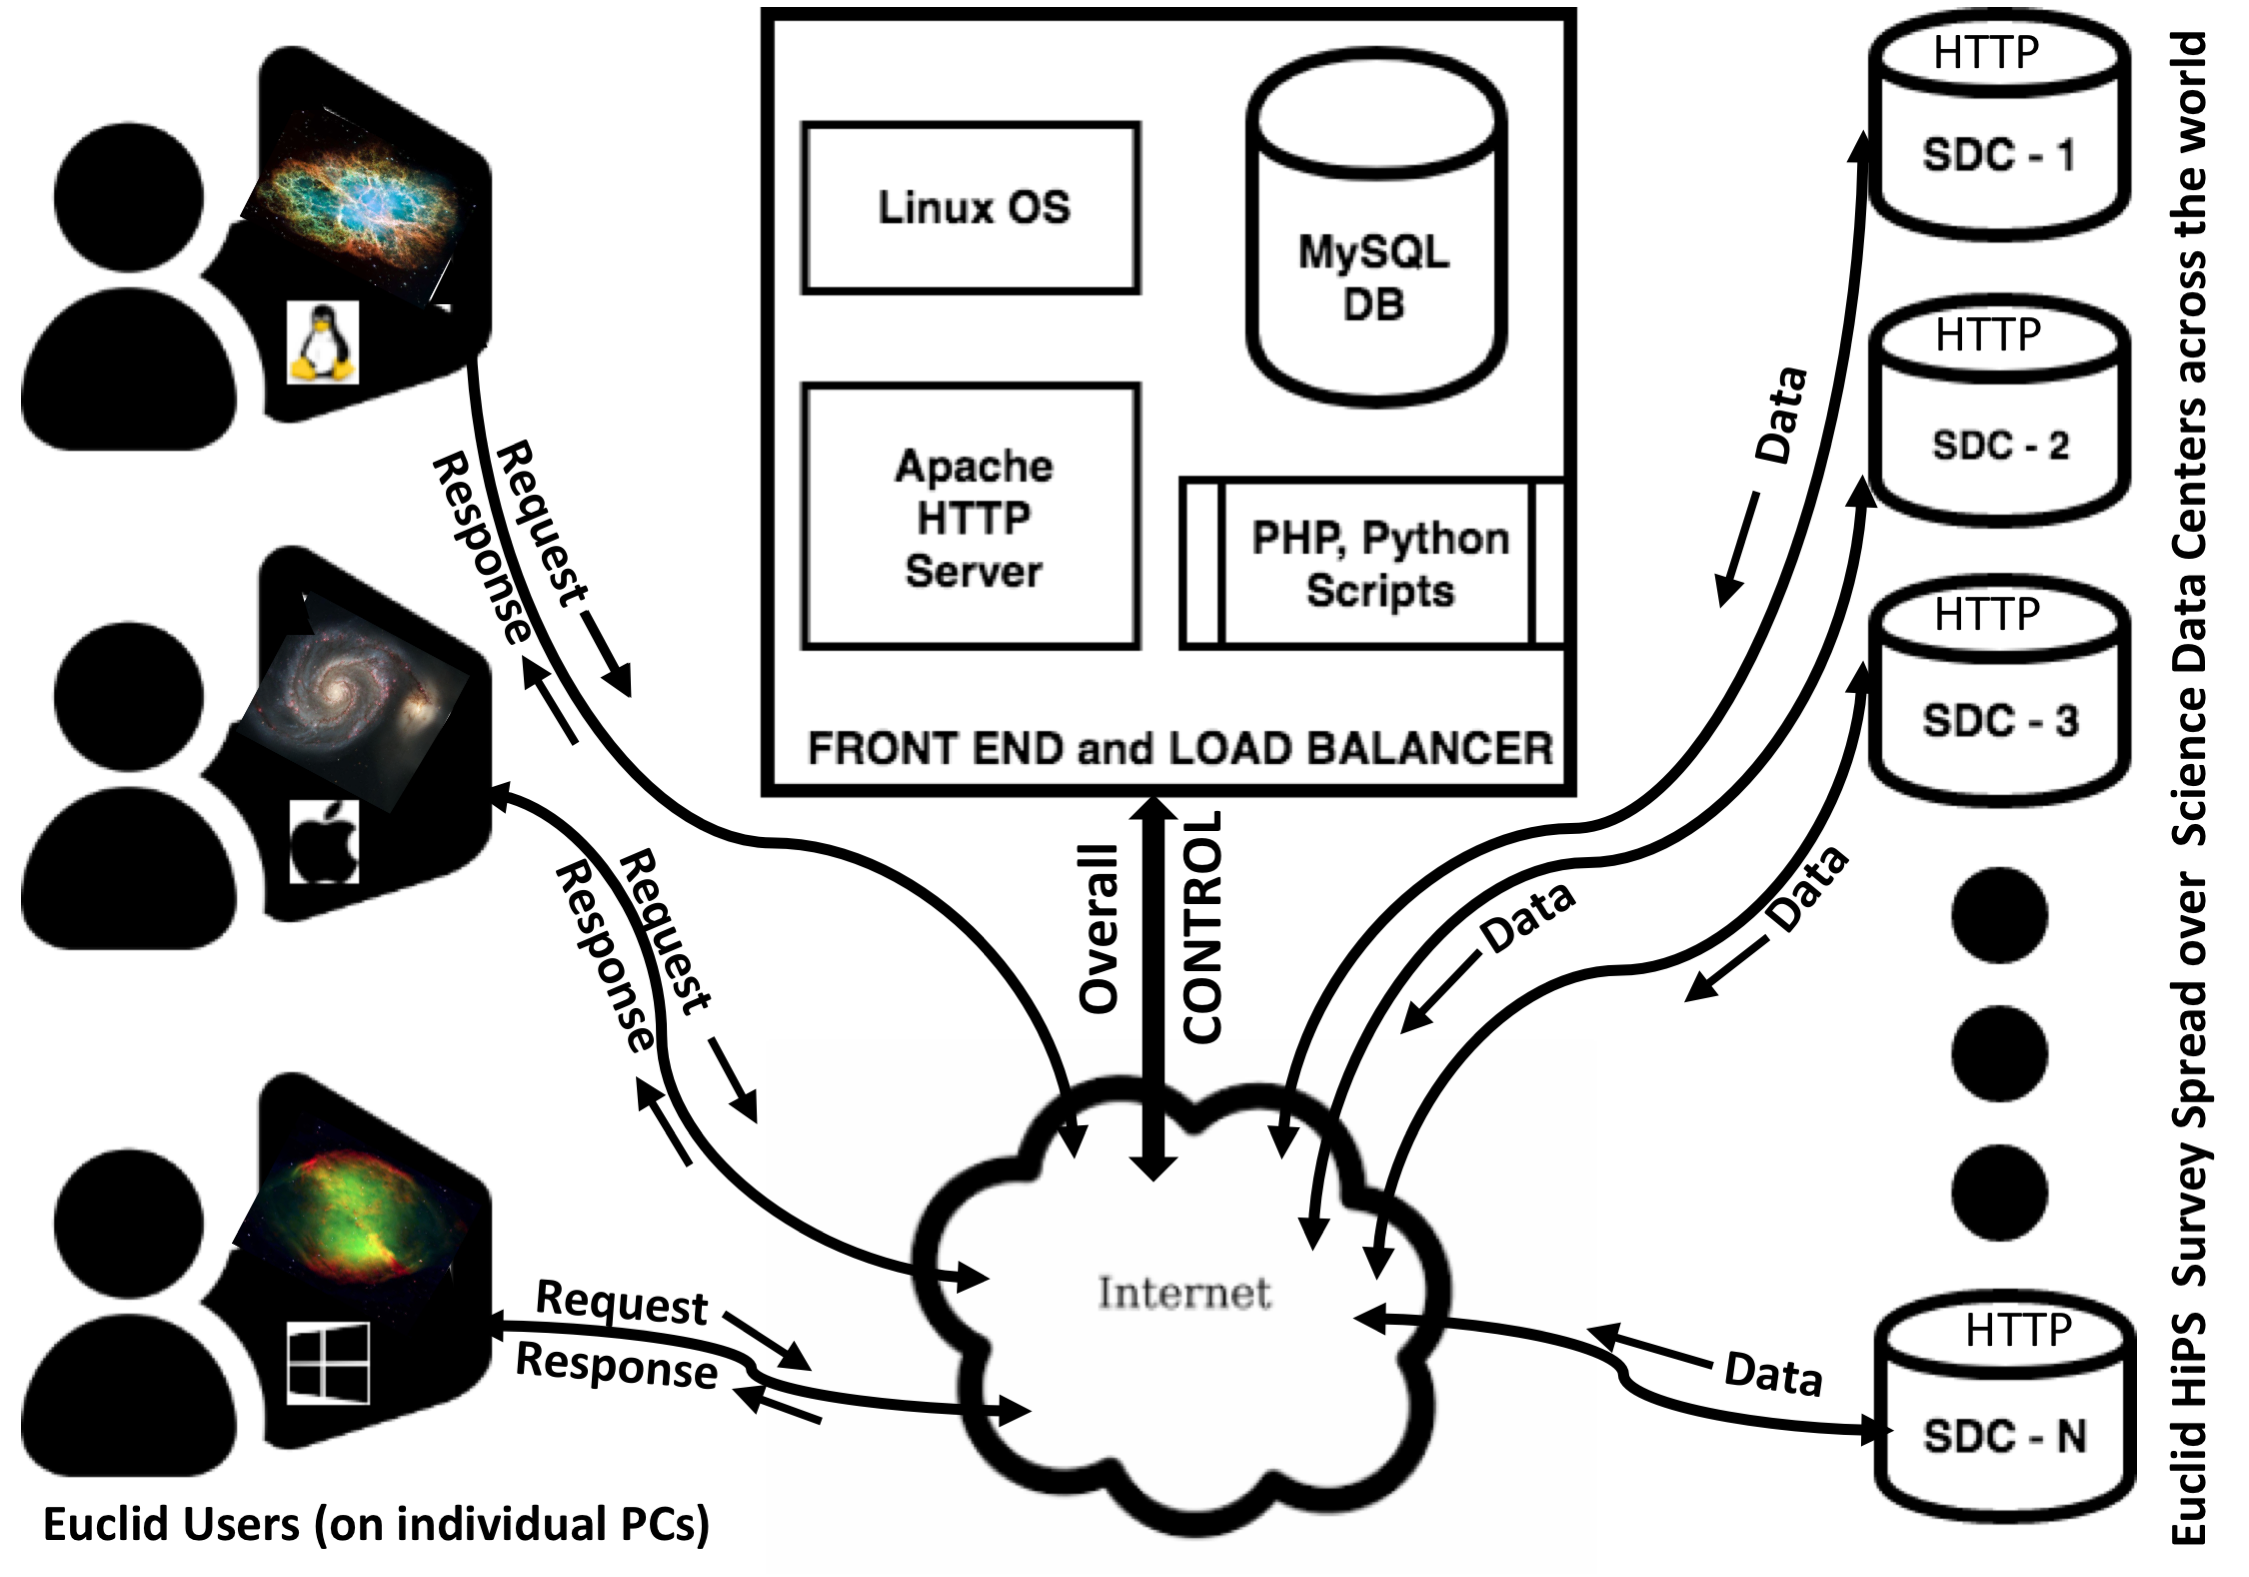
\includegraphics[width=\textwidth]{distributed_visualization_schema.png}
    \caption{An overall simple schematic of the distributed visualization framework in action. Using Aladin, several astronomers visualize their regions of interest (Euclid surveys) on their individual PCs\,(various OS). The FEN has the overall control and also acts as the first contact point for all Aladin requests. It may respond to a request by sending  the locally available information or  redirect Aladin to fetch it from a {\it{http}} server at an appropriate SDC\,(fully distributed mode set up), or itself send it after  fetching it from the SDC\,(reverse proxy set up).}
    \label{fig:dist_vis_schema}
\end{figure}

Our framework is based on the generic software LAMP stack model founded on four open source software components namely Linux, Apache, MySQL (and alternatives) and PHP (and alternatives). Figure\,\ref{fig:dist_vis_schema} shows the three main  constituents in the framework namely (i) Astronomers using Aladin at their PCs to remotely visualize Euclid surveys (ii) A FEN acts  as the main interface for Aladin requests and hosts the mandatory and recommended\,(optional) files necessary to initiate survey  visualization\,(e.g. properties, index.html, moc.fits etc.).  It has Linux operating system (e.g. Ubuntu, Scientific Linux etc.) with an listening Apache {\it{http}} server, a MySQL server/database and PHP/Python scripts.  The database contains the necessary entries to locate each survey file constituting  the entire survey (across all SDCs). The PHP/Python scripts dynamically handle incoming {\it{http}} requests and initiating appropriate action.  (iii) The SDCs collectively host the actual survey files/images including an apache {\it{http}} server listening to incoming requests.  %The survey images may be distributed across the SDCs in any desired manner (e.g. as per observation pointing, sky coverage etc.).

 

\begin{figure}[ht]
    \centering
%    \noindent\makebox[\textwidth]
   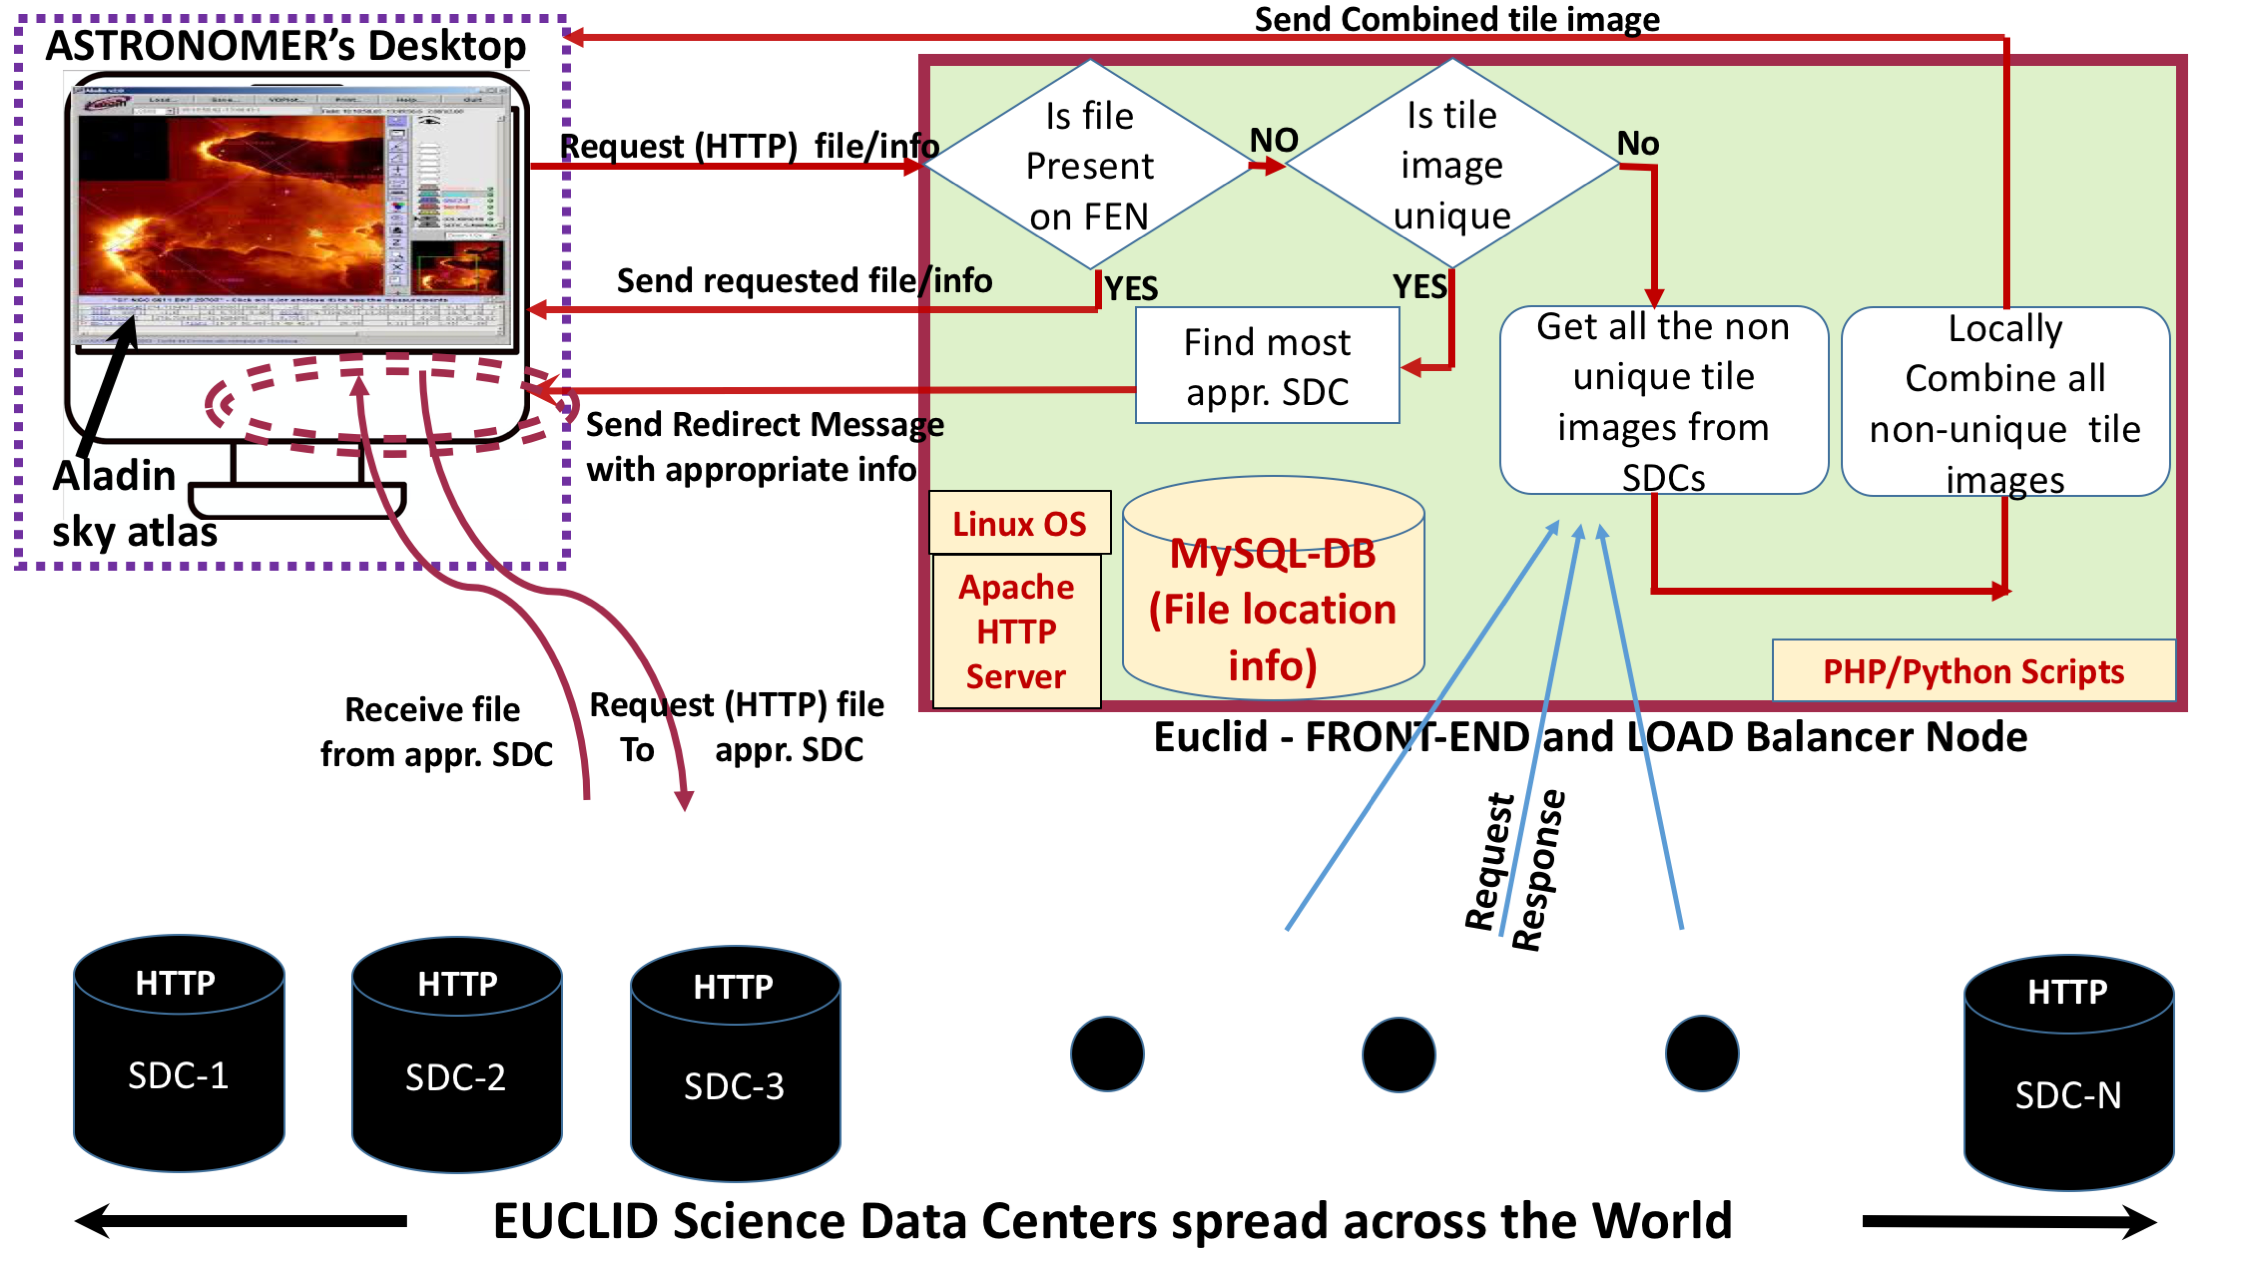
\includegraphics[width=\textwidth]{euclid_sweta_slide_DVisualization_Distributed_30Sep2019_v1_forpaper.png}
    \caption{A simplified flowchart depicting how a {\it{http}} request by Aladin\,(client) is handled when  the visualization framework is configured in fully distributed mode. All genuine Aladin requests can be appropriately responded as shown above and described in Sec.\ref{secn:arch_design}.}
    \label{fig:dist_vis_schema_flowchart}
\end{figure}

The visualization framework can be set up in two modes namely ($\bf{1.}$) fully distributed visualization mode and ($\bf{2.}$) a reverse proxy mode. Figure\,\ref{fig:dist_vis_schema_flowchart} shows a simplified flowchart for the fully distributed mode setup. An astronomer initiates survey visualization using Aladin from his PC. Aladin makes a {\it{http}} request for the desired information to the {\it{http}} server  on the FEN.  There could be (mainly) three possible  scenarios\,: ${\bf(a)}$\,the request is for one of the basic mandatory (or recommended) files (hosted at FEN) ${\bf(b)}$\,The requested file is unique and present at one or more SDCs and ${\bf(c)}$\,The requested file is non unique and present at one or several SDCs. Here the term unique refers to files which have only identical copies at one or more  SDCs. The term non-unique refers to a file present at multiple SDCs some of which contain non-identical information (e.g. same tile images but with different partial coverage). 

In case\,(a)\,the {\it http} server at FEN responds with the requested file. In case\,(b)\,a it responds with a {\it redirect message}  to Aladin with the details of the most appropriate SDC to where the request must be re-addressed. Aladin re-requests to the {\it{http}} server at the appropriate SDC which responds with the desired file. In case\,(c)\,a PHP script is instantiated which requests and receives all the non-unique instances of the requested file from the SDCs, combines them locally and responds with the resulting combined file to Aladin.  

In the fully distributed mode setup, the clients can directly communicate with SDCs while in the reverse proxy mode setup clients communicate only with FEN and the SDCs are shielded from direct access.   The fully distributed visualization mode  is network efficient since most of the actual data transfer to the clients happens  directly from the SDCs hosting it. The reverse proxy mode setup is convenient for overall monitoring and system security.

\section{Discussion, Conclusions and Future work}

We have successfully developed a distributed visualization framework with the aim of enabling users to visualize all sky HiPS surveys as if it  was stored locally on their individual PCs. 
%The only requirement at the astronomers end is to have a functional Aladin sky atlas and an internet connection.
It places no constraints on the inherent  capabilities of Aladin and on the SDCs including their heterogeneity in terms of their size, system design, operating system, file systems and intra-SDC bandwidth. An user on his PC screen can visualize either a small sky area at high angular resolution or a large sky area at low angular resolution given the limited number of screen pixels. Thus the visualization framework needs to transfer only a limited amount of data which can  be visualized at a given time. Every http request from all the users  is handled simultaneously (in parallel), automatically and independently including the data transfer due to stateless nature of the http protocol.  

The Euclid mission launch is scheduled for next year. The absence of  actual functioning SDCs posed a practical challenge for a test bed to carry out framework development. In view of this the present work has been carried using  {\it Virtual Machines} (\url{https://www.oracle.com/virtualization}) as  SDCs and the laptop as the FEN.  In order to evaluate performance, further tests and refinements we are  now implementing the visualization framework on OmegaCEN servers\,(\url{http://www.astro.rug.nl/~omegacen}) for the  Kilo-Degree Survey\,(KiDS). 
We plan  to document the installation steps (including server configurations and code) to publish it on {\it Gitlab} for open access.  We expect to make  further significant improvements by  exploring various options which include but are not limited to\,: NoSQL distributed data bases like  Apache Cassandra, NGINX {\it{http}} sever on SDCs,  key-value stores, replacing PHP scripts by daemon process, caching for network optimization, ELK stack with KIbana as Web-UI for integrated performance monitoring/fault detection. We also aim to implement the framework on cloud based storage at SURFsara.   The International Virtual Observatory Alliance\,(IVOA) is expected to play a critical role for future big truly international projects\,(e.g. SKA) where  single entities cannot efficiently tackle the {\it Big Data} volumes. In that context, we expect  our work would play  a useful role . 

\bibliography{example}  % For BibTex

% if we have space left, we might add a conference photograph here. Leave commented for now.
% \bookpartphoto[width=1.0\textwidth]{foobar.eps}{FooBar Photo (Photo: Any Photographer)}

%% https://arxiv.org/abs/1701.08158 This is the Euclid Data Challenges Paper by Andrey
\end{document}
